\documentclass{article}[12pt]
\usepackage{fullpage}
% Packages
\usepackage{amsfonts}
\usepackage{amsmath}
\usepackage{amsthm}
\usepackage{graphicx}


%\theoremstyle{plain}
\usepackage{amsmath,bm}

\newtheorem{lemma}{Lemma}
\newtheorem{claim}[lemma]{Claim}
\newtheorem{theorem}[lemma]{Theorem}
\newtheorem{corollary}[lemma]{Corollary}
\newtheorem{definition}{Definition}
\newtheorem{question}{Question}

\newcommand{\note}[1]{\par{\bf Note:}#1\par}
\newcommand{\notem}[1]{{\marginpar{\tiny #1}}}

\newcommand{\figline}{\rule{\textwidth}{1pt}}

%\newcommand{\proof}{\noindent{\bf Proof:} }
%\newcommand{\qed}{\rule{0.7em}{0.7em}}

\newcommand{\newmcommand}[2]{\newcommand{#1}{{\ifmmode {#2}\else\mbox{${#2}$}\fi}}}
\newcommand{\newmcommandi}[2]{\newcommand{#1}[1]{{\ifmmode {#2}\else\mbox{${#2}$}\fi}}}
\newcommand{\newmcommandii}[2]{\newcommand{#1}[2]{{\ifmmode {#2}\else\mbox{${#2}$}\fi}}}
\newcommand{\newmcommandiii}[2]{\newcommand{#1}[3]{{\ifmmode {#2}\else\mbox{${#2}$}\fi}}}

\newcommand{\E}[2]{{\bf E}_{#1}\left[ #2 \right]}
%\newcommand{\D}[2]{{\bf D}_{#1}\left[ #2 \right]}
\newcommand{\D}{{\cal D}}

\renewcommand{\P}[2]{{\bf P}_{#1}\left[ #2 \right]}
\newcommand{\reals}{\mathbb{R}}

\newcommand{\argmin}{\mbox{argmin}}
\newcommand{\argmax}{\mbox{argmax}}
\newcommand{\SP}[1]{{\cal P}^{#1}} % strictly positive function of
                                   % order i
\newcommand{\R}{R}      % Cumulative regret
\newcommand{\vR}{\mathbf{R}} %regret vector

\renewcommand{\r}{r}      % Instantaneuous regret
\newcommand{\state}{{\bf \Psi}}
\newcommand{\1}[1]{{\mathbf 1}\left[#1\right]} % point mass at #1

\newcommand{\pot}{\phi}
\newcommand{\potPQ}{\pot_{\learnerM,\adversM}}
\newcommand{\potLA}{\pot_{\l,\a}}
\newcommand{\finalPot}[1]{\pmb{\phi}_{#1}}
\newcommand{\finalPotT}{\finalPot{T}}
\newcommand{\finalPotR}{\finalPot{\realT}}
\newcommand{\upperpot}{\pot_{\learnerM}^{\downarrow}}
\newcommand{\upperpotb}{\pot_{\learnerMb}^{\downarrow}}
\newcommand{\upperpotd}{\pot_{\learnerMd}^{\downarrow}}
%\newcommand{\upperpotj}{\pot_{\learnerM(j)}^{\downarrow}}
\newcommand{\upperpotMdk}{\pot_{\learnerMdk}^{\downarrow}}
\newcommand{\upperpotMdj}{\pot_{\learnerMdj}^{\downarrow}}


\newcommand{\lowerpot}{\pot_{\adversM}^{\uparrow}}
\newcommand{\lowerpotb}{\pot_{\adversMb}^{\uparrow}}
\newcommand{\lowerpotd}{\pot_{\adversMd}^{\uparrow}}
\newcommand{\lowerpotj}{\pot_{\adversM(j)}^{\uparrow}}
\newcommand{\lowerpotMdk}{\pot_{\adversMdk}^{\uparrow}}
\newcommand{\lowerpoteven}{\lowerpot_{\evensplit}}

\newcommand{\realT}{\mathcal{T}}  % the final time for the real-time
% game
\newcommand{\Tset}[1]{\pmb{T}_{#1}}
\newcommand{\Ilat}[1]{\pmb{I}_{#1}}
\newcommand{\Klat}[1]{\pmb{K}_{#1}}
\newcommand{\score}{\Phi}
\newcommand{\upperscore}[1]{\score_{#1}^{\downarrow}}
\newcommand{\lowerscore}[1]{\score_{#1}^{\uparrow}}

\newcommand{\upperscoreM}{\upperscore{\learnerM}}
\newcommand{\upperscoreMd}{\upperscore{\learnerMd}}
\newcommand{\upperscoreMdk}{\upperscore{\learnerMdk}}

\newcommand{\lowerscoreM}{\lowerscore{\adversM}}
\newcommand{\lowerscoreMd}{\lowerscore{\adversMd}}
\newcommand{\learnerM}{P}
\newcommand{\learnerMb}{P_I}
\newcommand{\learnerMd}{P_D}
\renewcommand{\l}{\learnerM}
\newcommand{\learnerMdk}{P_{D(k)}}
\newcommand{\learnerMdj}{P_{D(j)}}


\newcommand{\legalLearner}{{\cal L}}

\newcommand{\adversM}{Q}
\newcommand{\adversMb}{Q_I}  %Integer time game
\newcommand{\adversMd}{Q_D}  % Discrete time game
\newcommand{\adversMdk}{Q_{D(k)}}  %Discrete time game with step of
                                %size 2^{-k}


% \renewcommand{\a}{\adversM}
%\newcommand{\legalAdversary}{{\cal A}}
\newcommand{\agloss}{v}
\newcommand{\Bias}{B}
\newcommand{\deltat}{\Delta t}

\newcommand{\diffweight}{\l^d}   % learner strategy based on taking a difference
\newcommand{\upperpotdiff}{\upperpot_{\diffweight}}


\newcommand{\Binom}{\mathbb{B}}
\newcommand{\radsum}{\Binom(s_1,\ldots,s_T)}
\newcommand{\var}{\mbox{Var}}
\newcommand{\V}{V}


\newcommand{\at}[1]{\left\{ \left. #1
    \right|_{\begin{tiny}\begin{matrix}
          \tau,\rho=\\t_i,\R \end{matrix} \end{tiny}}
    \pot(\tau,\rho)\right\}}
\newcommand{\att}[1]{\left\{ \left. #1  
\right|_{\begin{tiny}\begin{matrix} \tau,\rho=\\t_i+g \deltat_i,\R_i+g
      r_i \end{matrix} \end{tiny}}
\pot(\tau, \rho)\right\}}


\newcommand{\atI}[1]{\left\{ \left. #1  
\right|_{\begin{tiny}\begin{matrix}
      x,y=\\x_0,y_0 \end{matrix} \end{tiny}}
f(x,y) \right\}}
\newcommand{\atII}[1]{\left\{ \left. #1
\right|_{\begin{tiny}\begin{matrix}
      x,y=\\x_0+t\Dx,y_0+t\Dy \end{matrix} \end{tiny}}
f(x,y) \right\}}


\newmcommandi{\paren}{\left({#1}\right)}
\newmcommandi{\brac}{\left[{#1}\right]}




\title{An Optimal potential-based hedging algorithm}
\author{Yoav Freund}
\begin{document}

\maketitle
\begin{abstract}
We study a family of potential functions for online learning. We show
that if the potential function has strictly positive derivatives of
order 1-4 then the min-max optimal strategy for the adversary is Brownian
motion. Using that fact we analyze different potential functions and
show that the Normal-Hedge potential is optimal.
\end{abstract}


\section{Introduction}

Online prediction with expert advise has been studied extensively over
the years and the number of publications in the area is vast (see
e.g.~\cite{vovk1990aggregating, feder1992universal,
  littlestone1994weighted, cesa1997use, cesa2006prediction}.

Here we focus on a simple variant of online prediction with expert
advice called {\em the decision-theoretic online learning game}
(DTOL)~\cite{freund1997decision}, we  consider the {\em
  signed} version of the online game.

DTOL is a repeated zero sum game between a {\em learner} and an {\em
  adversary}. The adversary controls the losses of $N$ experts, or
actions, while the learner controls a distribution over the actions.
~\\
Iteration $t=1,\ldots,T$ of the game consists of the following steps:
\begin{enumerate}
    \item The learner chooses a distribution $P_j^t$ over the
      actions $j \in \{1,\ldots,N\}$. 
    \item The adversary chooses an {\em instantaneous loss} for each
      of the $N$ actions: \\
      $l_j^t \in [-1,+1]$ for $j \in \{1,\ldots,N\}$.
    \item The learner incurs an {\em instantanous expected loss} defined as
      $\ell^t = \sum_{j=1}^N P_j^t l_j^t$
\end{enumerate}

Using standard notation we denote the {\em cumulative loss} of
action $j$ for times $1,\ldots,T$ by $L^T_j = \sum_{t=1}^T l_j^t$.
Similarly, we denote the {\em cumulative loss} of the learner by
$L_\ell^T = \sum_{t=1}^T \ell^T$.
%The {\em instantaneous regret} of
%the learner with respect to action  $j$ is defined as
%$r_j^t = \ell^t-l_j^t$.
The {\em cumulative regret} of the learner
with respect to action $j$ is $\R_j^T = \sum_{t=1}^T r_j^t =
L_\ell^T -L_j^T $. Finally, for any $0\leq \epsilon \leq 1$ we define the $\epsilon$ regret
to $R^T_\epsilon$ to be value $v$ such that the
fraction of values of $\R_j^T$ that are smaller than $v$ is at most
$\epsilon N$.

The goal of the learner is to minimize the maximal regret at time $T$
$R_{\epsilon}^T \doteq \max_j \R_j^T = L_\ell^T - \min_j L_j^T$.
The goal of the adversary is to maximize $R_{\epsilon}^T$.

Our goal is to identify algorithms that improve over known bounds of the
form $O(\sqrt{T \ln \frac{1}{\epsilon}})$.
{\bf Needs comparison to existing results, NormalHedge, Squint, square
loss bounds}

We are interested in bounds the hold simultanously for all values
of $\epsilon$. Denote the distribution over regrets at some fixed
iteration by $\mu$. We say that the distribution $\mu$ satisfies the regret function $B$ if

\begin{definition}[Simultanous regret
  bound] \label{def:unif-regret-bound}
  Let $B: \reals \to [0,1]$ be a non-increasing function which maps
  regret bounds to probabilities.
  
  A distribution over regrets $\mu$ is simultanously bounded by $B$ if
  \[
    \forall r \in \reals \;\; \P{\R \sim \mu}{\R \geq r} \leq B(r)
  \]
Where $B: \reals \to [0,1]$ is a non-increasing function.
\end{definition}

Our main tool for designing algorithms and proving bounds is potential
functions.

We say that  A distribution over regrets $\mu$ satisfies
the potential function $\pot$ if 
%We say that the bound $B_1$ dominates $B_2$ if $\forall r  B_1(r) \leq
%B_2(r)$ and $\exists r B_1(r) <B_2(r)$

\begin{definition}[Average potential bound] \label{def:aver-potential-bound}
  A distribution over he reals $\mu$ satisfies the average
  potential function $\pot$ if
  $$\E{\R \sim \mu}{\pot(\R)} \leq 1$$
  Where $\pot: \reals \to \reals^+$ is a non decreasing function. 
\end{definition}

\begin{theorem}
 A distribution $\mu$ is simultanously bounded by $B$ if and only
 if it satisfies the average potential bound with $\phi(\R) = B(\R)^{-1}$
\end{theorem}

Unlike uniform regret bounds, that are rather opaque, one can easily
write a single step backward recursion for potentials. In other words,
given a potential function at iteration $t$, one can construct
potential functions for iteration $t-1$. This povides a way 
for optimizing the potential function.

The original DTOL game does not seem to have min-max
strategies. However, in an extended version of the game we can
characterize min-max strategies. The extended game provides the
adversary with additional possibilities, but not the learner. In other
words, the standard game is more restrictive to the adversary, which
means that upper bounds on the regret for the extended game also hold
for the restricted game.

\begin{itemize}
\item min-max for known $T$
\item Almost min/max for unknown $T$
\item Simultanously for all $\epsilon$
\item Replacing $T$ with $V_T$
\item Interpretation of the limit game.
\end{itemize}

\subsection{Some known Bounds}
Zero-order bounds on the regret ~\cite{freund1999adaptive} depend only on $N$
and $T$ and typically have the form
\begin{equation} \label{eqn:0-order-bound}
  \max_j \R_j^T < C E \sqrt{T \ln N}
\end{equation}
for some small constant $C$ (typically smaller than 2).
These bounds can be extended to infinite sets of experts by defining
the $\epsilon$-regret of the algorithm as the regret with respect to
the best (smallest-loss) $\epsilon$-percentile of the set of experts.

this replaces the bound~(\ref{eqn:0-order-bound}) with 
\begin{equation} \label{eqn:0-epsilon-order-bound}
  \max_j \R_j^T < C E \sqrt{T \ln \frac{1}{\epsilon}}
\end{equation}

Lower bounds have been proven that match these upper bounds up to a
constant. These lower bounds typically rely on constructions in which
the losses $l_j^i$ are chosen independently at random to be either
$+1$ or $-1$ with equal probabilities.

Several algorithms with refined upper bounds on the regret have been
studied. Of those, the most relevant to our work is a paper by 
Cesa-Bianchi, Mansour and
Stoltz~\cite{cesa2007improved} on second-order regret bounds.
The bound given in Theorem~5 of ~\cite{cesa2007improved} can be
written, in our notation, as:
\begin{equation} \label{eqn:2nd-order-bound}
  \max_j \R_j^T \leq 4\sqrt{V_T \ln N} +2 \ln N +1/2 
\end{equation}
Where
\[
  \var_i = \sum_{j=1}^N P^i_j (l_j^i)^2 -  \left( \sum_{j=1}^N P^i_j
    l_j^i \right)^2 \mbox{ and } \V_T= \sum_{i=1}^T \var_i
\]

A few things are worth noting. First, as $|l_j^i|\leq 1$,
$\var_j\leq 1$ and therefor $V_T\leq T$. However $\V_T/T$ can be
arbitrarily small, in which case inequality~\ref{eqn:2nd-order-bound}
provides a tighter bound than ~\ref{eqn:0-order-bound}. Intuitively,
we can say that $\V_T$ replaces $T$ in the regret bound. This paper
provides additional support for replacing $T$ with $\V_T$ and provides
lower and upper bounds on the regret involving $\V_T$.

\subsection{Potential Functions}
A common approach to design online learning algorithms is to define a
{\em potential function}.  The potential function is a continuous
positive and increasing function of the regret $\R_j^i$. A popular
potential function is the exponential function which has the form
$\pot(\R_j^i) = \exp(\eta \R_j^i)$ where $\eta>0$ is the {\em learning rate}. The central
quantity n the design and analysis of potential based online-learning algorithms is
the {\em average potential} or {\em score}, defined as:

$$\score^t = \frac{1}{N} \sum_{j=1}^N \pot_j^t$$

Proving regret bounds are based on combining the upper and lower
bounds on the score
\begin{itemize}
\item {\bf Upper bound}: If the cumulative loss of the best expert is
  small then the score is small.
\item {\bf lower bound}: If the cumulative loss of the learning algorithm is large
then the score is large.
\end{itemize}

Most of the papers on potential based online algorithms consider
one or a few potential functions. Most common is the exponential
potential, but others have been considered~\cite{cesa2006prediction}.
A natural question is what is the difference between potential
functions and whether some potential function is ``best''.

In this paper we consider a large set of potential functions,
specifically, potential functions that are strictly positive and have
strictly positive derivatives of orders up to four. The exponential
potential and the NormalHedge potential~\cite{chaudhuri2009parameter,luo2015achieving}
are member of this set. 

To analyze these potential functions we define a slightly different
game, which we call a ``potential game''. In this game the primary
goal of the learner is not to minimize regret, rather, it is to
minimize the final score $\score^T$. To do so
we define potential functions for intermediate steps: $0 \leq t
<T$.\footnote{The analysis described here builds on a long line of
  work. Including the Binomial Weights algorithm and it's
  variants~\cite{cesa1996line,abernethy2006continuous,abernethy2008optimal}
  as well as drifting games~\cite{schapire2001drifting,freund2002drifting}.}


There are two potential functions one corresponding to the
learner's strategy, denoted $\upperpot$, which defines an upper bound
on $\score^T$ and one to the adversary's strategy, denoted
$\lowerpot$, which defines a lower bound on $\score^T$. We show that
good strategies for the learner and for the adversary correspond to
two slightly different random walks. However, the upper bound and
lower bounds derived this way do not match. 
To find min-max matching strategies, we need to move to variable
time steps.

\subsection{Variable time steps}
The second order bounds of~\cite{cesa2007improved} show that, in some
contexts, the time parameter $t$ can be replaced by a variance-type
parameter $\V_T= \sum_{i=1}^T \var_i$. This corresponds to a
significant tightening of the bound. For example if instead of $l_j^i
\in [-\epsilon,+\epsilon]$, then $\V_T = T\epsilon^2$, and if we set
$T=\epsilon^{-2}$ we get n upper bound on the regret that does not
depend on $T$. The idea is to replace $T$ with $V_T$ in the definition
of the upper and lower potentials. Which is what we do in
Section\ref{sec:discrete}.

In that variant of the potential game the adversary chooses the
``real-time'' step at each iteration. Surprisingly, it turns out that
the adversary's preference is to make the time steps as small as
possible (but not zero). Combining the random walk strategy with the
infinitesimal time step, we arrive at a strategy that is define by
Brownian motion, or a Wiener process. Even more surprisingly, the
strategy of the learning at this limit corresponds to the same
Brownian motion. In other words, we have a min-max characterization of
DTOL.

\paragraph*{The rest of the paper is organized as follows}
In Section~\ref{sec:preliminaries} we provide some basic definitions.
In Section~\ref{sec:integer} we describe the potential game in the standard
integer time case and prove some upper and lower bounds for this
case. In Section~\ref{sec:discrete} we define a the discrete time
game, where time advances are real valued and finite. The core of our
argument, which is based on the theory of ``divided-differences''
appears in Section~\ref{sec:smallsteps}. In
Section~\ref{sec:continuous} we define the continuous time limit of
the game. In Section~\ref{sec:self-consistent} we show that optimal
any-time potential functions correspond to the solution of the
kolmogorov Backwards differential equation, and show the Exponential weights and
NormalHedge are solutions for that Equation. Finally, in
Section~\ref{sec:NormalHedge}
we argue that NormalHedge is the best possible potential function.


\iffalse
\subsubsection*{Our Contributions}
\begin{itemize}
\item We characterize the min/max strategies for 
  potential functions that have strictly positive derivatives up to
  order four.
\item We show that the optimal adversarial strategy for all of
  these potential functions is a strategy corresponding to
  Brownian motion.
\item We show that $V_T$ replaces $T$ for any of these games.
\item  We show that all potential functions that satisfy a particular
  partial differential equations yield min/max solutions to the
  potential game.
\item We show that both the exponential weights algorithm and
  NormalHedge are solutions to the PDE.
  \item We show that NormalHedge provides the best possible regret bounds.
\end{itemize}

In this paper we extend and refine the analysis of the potential
function to
provide a min/max analysis for a large set of potential functions. We
then show that NormalHedge is, in a strong sense the best of those
potential functions.

Our analysis is based on three ideas that are listed below.
\begin{itemize}
    \item {\bf Potential games:} We focus on the potential function, rather than on the problem of minimizing regret. In other words, we define a new game, in which the goal of the learner is to minimize  the final average potential.
    \item {\bf Experts as a probability space:} Instead of restricting the game to $N$ strategies, we allow the set of strategies to be an arbitrary probability space. This allows the adversary the following simple but powerful strategy.  At each iteration $i$ the adversary splits each one of the strategies into two equal parts, once part incurs loss $-1$ and the other loss $+1$. In other words, at iteration $i$ there are $2^i$ strategies, each corresponding to a sequence in $\{-1,+1\}^i$. It is intuitively clear that the instantaneous loss of the learner is always zero, regardless of it's choice of $P$.
    \item {\bf Reducing the time step and continuous time:} Regret bounds of the form $C\sqrt{T \ln N}$ are tight for the case in which the adversary assigns losses of $\pm 1$ with equal probabilities.
    Suppose however, that the adversary produces the exact same sequence of losses, but divides the range of each loss by 2. In this case the losses and the regrets will all be divided by two, but the bound will remain the same! This suggest that defining $T$ as the number of iterations in the game leaves some slack. To remedy this situation we let time take on real values such that $t_{i+1}-t_i \leq 1$. At the same time we 
    allow the adversary to declare, before each iteration, the range $[-s_i,+s_i]$ for the losses, in which case the following time would be 
    $t_{i+1}=t_i +s_i^2$. Surprisingly, we find out that for a large set of potential functions, the preference of the adversary is to make $s_i$ as small as possible, making iterative game into a continuous time game and the adversarial strategy to be Brownian motion.
\end{itemize}

\fi

\section{Preliminaries} \label{sec:preliminaries}
The game takes place on the set $(t,\R) \in [0,T] \times \reals$,
where $t$ corresponds to time, $T$ correspond to the
time at the end of the game (i.e. this is a bounded horizon game where the
horizon is known to both players. $\R$ corresponds to (cumulative) regret).

As in the DTOL setting, an strategy (or expert) correspond to a sequence of instantaneous losses. 
However, unlike the standard DTOL the number of strategies is not finite or known in advance. In DTOL the {\em state} of the learning process is defined by the 
by the regret of each of the $N$ strategies: $\langle \R_1(t),\ldots,\R_N(t) \rangle$. In order to represent the regret of a potentially
uncountable set of strategies we define the state as a  distribution over possible regret values.
Thus the {\em state} of the game at time $t$ is a distribution (finite measure) over the real line, denoted $\state(t)$. 
We denote by $\R \sim \state(t)$ a random regret $\R$ that is chosen according to the state at time $t$. 

The transition from an $N$ dimensional vector to a distribution is {\em central} to our analysis. The adversarial strategy we use splits each one of the strategies at time  $t$ into two: one half has instantaneous regret of $+1$ and the other instantaneous regret of $-1$. The adversary might not be able to use
this strategy when the number of strategies is finite. If there is only one strategy with cumulative regret $\R$ then that strategy cannot, by definition, be split into two. Giving the adversary more possibilities allows us to narrow the gap between upper and lower bounds.

The initial state $\state(0)$ is a point mass at $\R=0$. 
The state $\state(t)$ is defined by $\state(t_{i-1})$ and the choices made
by the two players as described in the next section.

The score of the game is defined by $\state(T)$ and a function called the {\em final potential function}
$\finalPot(\R)$ that is fixed a-priori and is known to both players.  The final score of the game is defined as
\begin{equation} \label{eqn:FinalExpectedValue}
  \score(T) =\E{\R \sim \state(T)}{\finalPot(\R)}
\end{equation}
The goal of the learner is to minimize $\score(T)$ and the goal of
the adversary is to maximize it.

We assume that the function is {\em strictly positive of degree $k$}, which is defined as follows:
\begin{definition}[Strict Positivity of degree $k$]
A function $f:\reals \to \reals$ is strictly positive of degree $k$, 
denoted $f \in \SP{k}$ if the derivatives of orders 0 to $k$:  
$f(x), \frac{d}{dx}f(x), \ldots, \frac{d^k}{dx^k}f(x)$ exist and are strictly positive.
\end{definition}

A simple lemma connects an upper bound on any score function in $\SP{1}$ with a bound on the regret.
\begin{lemma}
Let $\finalPot(\cdot) \in \SP{1}$, $\score(T) \leq U$ and $\epsilon=\P{\R \sim
  \state{t}}{\R >\R'}$ be the probability of the set of actions with
respect to which the regret is larger than $\R'$ Then

then the regret of the algorithm relative 
to the top $\epsilon$ of the strategies is upper bounded by
\[
  \finalPot(\R') \leq U/\epsilon
\]
\end{lemma}

For the rest of the paper we will focus on strategies for upper and lower bounding $\score(T)$. We will come back to the relationship between the bounds on $\score(T)$ and the regret at the end of the paper, where we will argue that NormalHedge is, in a sense, the best possible potential function.

We will first consider the standard setting where time corresponds to
the natural and is equal to the iteration number $t_i=i$. Later we
expand the game the $t_i$ can take on any real value in $[0,T]$ under
the condition that $t_{i-1} \leq t_i \leq t_{i-1}+1$.

\section{Integer time game} \label{sec:integer}
We start with the standard setup in which time corresponds to the
natural numbers, $t_i=i$. to simplify notation we will use the
iteration number $i$ instead of time.

Connecting this back to decision theoretic online learning
(DTOL~\cite{}). The state $\state(i)$ corresponds to the distribution
over the regret values of the experts on iteration $i$. Note that here the set of
experts is allowed to be be un-countably infinite. In particular the
adversary can assign to the experts with regret $x$ at iteration $t$
an arbitrary distribution of losses in the range $[-1,+1]$.

The game is defined by three parameters:
\begin{itemize}
\item $T$ : The number of iterations
\item $\state(0) = \delta(0)$ is the initial state of the game which
  is a point mass distribution at 0. 
\item $\finalPot(\R)$ : The function that is in $\SP{2}$.
\item $0<c \leq 1$ - An upper bound on aggregate loss (loss of the master)
  in a single iteration. Note that the cumulative aggregate loss is at
  most $cT$. Note that $c=1$ is always satisfied and eliminates the
  constraint.
\end{itemize}

The transition from $\state(i)$ to $\state(i+1)$ is  defined by the
choices made by the adversary and the learner.

\begin{enumerate}
\item The learner chooses weights. Formally, this is
  a distribution over $\R \in \reals$: $\learnerM(i)$.
\item The adversary chooses the losses of the strategies. Formally 
  this is a mapping from $\reals$ to distributions
  over $[-1,+1]$: $\adversM(i): \reals \to \Delta^{[-1,+1]}$. We use
  $l \sim \adversM(i,\R)$ to denote the distribution over the
  instantaneous loss associated with iteration $i$ and regret $\R$.
\item The aggregate loss (also called ``the loss of the master") is
  calculated:
  \begin{equation} \label{eqn:agg-loss-complex}
  \ell(i)=\E{\R \sim \state(i)}{\learnerM(i,\R) \E{l \sim \adversM(i,\R)}{l}}
  \end{equation}
  
  The adversary is constrained to $\adversM$ such $|\ell(i)| \leq c$. 
  We define the {\em bias} at $(i,\R)$ to be  $\Bias(i,\R) \doteq \E{l
    \sim \adversM(i,\R)}{l}$ which allows us to rewrite
  Eqn~(\ref{eqn:agg-loss-complex}) as
  \begin{equation} \label{eqn:aggregate-loss}
    \ell(i)=\E{\R \sim \state(i)}{\learnerM(i,\R) \Bias(i,\R)}
  \end{equation}
  note that $\Bias(i,\R)$ is in $[-1,1]$ and that $\ell(i)$ is the mean
  of $\Bias(i,\cdot)$. Note also that $-1-c \leq y-\ell(i) \leq 1+c$
  corresponds to the instantanous regret. In the integer game, setting
  $c \geq 1$ is equivalent to placing no restriction on $\ell(i)$.
  
\item The state is updated. 
  \begin{equation} \label{eqn:state-update}
    \state(i+1) = \E{\R \sim \state(i)}{\R \oplus  \adversM(i,\R)}
    \ominus \ell(i)
    \end{equation}
  Where $\adversM(i,\R)$ is the distribution of the losses of experts
  that are at location $\R$ after iteration $i-1$. $\R \oplus
  \adversM(i,\R)$ is the same distribution shiften right by the amount
  $\R$. $ \E{\R \sim  \state(i-1)}{\cdot}$ indicates the expectation over distribution,
  yealding a new distribution. Finally $\ominus \ell(i)$ is a shift
  left of the resulting distribtion according to the aggregate loss. 
\end{enumerate}

The final score is the mean of the potential according to the final
state, as given in
Equation~(\ref{eqn:FinalExpectedValue})
\begin{equation}
  \score(T) =\E{\R \sim \state(T)}{\finalPot(\R)}
\end{equation}
The goal of the learner is to minimize the final score and the goal of
the adversary is to maximize it.
\subsection{Results for integer time game}

We prove two results for the integer game. One is a strategy for the
adversary that guarantees a lower bound on $\score(T)$ for any
strateyg of the learner,  the other is a strategy for the learner that
that guarantees an upper bound on $\score(T)$.

We use $B(n,s)$ to denote the binomial distribution that assigns
probability ${n \choose i} 2^{-n}$ to the point $(2i-n)s$ for
$i=0,\ldots,n$

\begin{theorem}
  ~\\
  \begin{itemize}
    \item
    There exists a strategy for the adversary such that for any strategy
    of the learner, $$\score(T) \geq \E{\R \sim B(T,1)}{\pot(T,\R)}$$
  \item
    There exists a strategy for the learner such that for any strategy
    of the adversary, $$\score(T) \leq \E{\R \sim B(T,1+c)}{\pot(T,\R)}$$
  \end{itemize}
\end{theorem}

\subsection{Analysis of the integer time game}

The final potential $\finalPot(\R)$ is part of the setup of the
game. We will extend the notion of the potential to earlier steps of
the game.

More specifically, we associate with any learner strategy an {\em
  upper potential} for the game and with any adversarial strategy a
{\em lower potential} for the game. When the upper and lower
potentials are equal, the associated strategies are min/max optimal.

We describe the upper potential, the lower potential
description is the same other than the learner and the adversary
are switched. Let $\l$ denote a learner
strategy and $\a$ denote an adversarial strategy. A legal strategy is
any mapping from sequences of actions (of both players) at previous steps to an
action for the current step. We will denote the set of all legal
strategies for the learner by $\legalLearner$, and for the adversary
by $\legalAdversary$. Let $\l$ and $\a$ be strategies for learner and
adversary respectively and $\state(i) = \delta(\R)$ defines a game
that starts at iteration $i$ with a state that is a point mass at
$\R$.
Then $\score(\l,\a,i,\R)$ is the final score if the game starts at
iteration $i$ with state $\state(i) = \delta(\R)$ and the players use
strategies $\l,\a$ respectively.

The upper potential for learner strategy $\l$ is defined as
\[
  \upperpot(\l,i,\R) = \sup_{\a \in \legalAdversary}\score(\l,\a,o,\R)
\]

\subsection{Strategies for integer time game}

Consider the states at two consecutive iterations $\state(i-1),\state(i)$.
Suppose that $\pot(i,\R)$, the value function for iteration $i$ is fixed.
We say that $\lowerpot(i-1,\R)$ is a lower bound on the value at iteration
$i-1$ if there is exists an adversarial strategy $\adversM^*$ such that
for any strategy of the learner $\learnerM$, 
$$ \E{\R \sim \state(i-1)}{\lowerpot(i-1)} \leq \E{\R \sim \state(i)}{\pot(i)}$$
Similarly, $\upperpot(i-1,\R)$ is an upper potential if there exists a
learner strategy $\learnerM^*$ such that for any adversarial strategy
$\adversM$,
$$ \E{\R \sim \state(i-1)}{\upperpot(i-1)} \geq \E{\R \sim \state(i)}{\pot(i)}$$


\begin{lemma} \label{lemma:adversary-prefers-extremes}
 Suppose $\lowerpot(i,\R)$ is strictly convex with respect to  $\R$.
Let ${\cal Q}(i-1,\R,\Bias)$ be the set of adversarial strategies 
$\adversM(i-1,\R)$ that have bias
$\Bias=\Bias(i-1,\R)= \E{y \sim \adversM(i-1,\R)}{y}$ then the
strategy in ${\cal Q}(i-1,\R,\Bias)$ that is best for the adversary is
\begin{equation} \label{eqn:adv-strat-p}
  \adversM^p(i-1,\R) =
  \begin{cases}
    +1 & \mbox{ w.p. } \frac{1+\Bias}{2}\\
    -1 & \mbox{ w.p. } \frac{1-\Bias}{2}\\
  \end{cases}
\end{equation}

\begin{equation} \label{eqn:value-iteration-lower-recursion}
  \lowerpot(i-1, \R) = p \lowerpot(i,\R+1) + (1-p)\lowerpot(i,\R-1)
\end{equation}
which is strictly higher than $\lowerpot(i-1,\R)$ for any other
distribution in ${\cal Q}(i-1,\R,\Bias)$. In addition,
$\lowerpot(i-1, \R)$ is strictly convex.
\end{lemma}


In the next lemma we describe strategies for the adversary and the
learner and prove upper and lower bounds on the potential that they
guarantee.

\begin{lemma} \label{lemma:first-order-bound}
  If $\pot(i,\R)$  is CIC then
  \begin{enumerate}
    \item The adversarial strategy
      \begin{equation} \label{eqn:adv-strat}
      \adversM^{1/2}(i-1,\R) =
      \begin{cases}
        -1 & \mbox{ w.p. } 1/2\\
        +1 & \mbox{ w.p. } 1/2
      \end{cases}
    \end{equation}
    Guarantees the lower potential
 \begin{equation} \label{eqn:value-iteration-lower}
   \lowerpot(i-1, \R) = \frac{\pot(i,\R+1) + \pot(i,\R-1)}{2}
 \end{equation}
   
    \item The learner strategy:
      \begin{equation} \label{eqn:learner-strat-1}
      \learnerM^1(i-1,\R) = \frac{1}{Z} \frac{\pot(i,\R+1+c) - \pot(i,\R-1-c)}{2}
      \end{equation}
      Where $Z$ is a normalization factor
      $$Z = \E{\R \sim \state(i)}{\frac{\pot(i,\R+1+c) - \pot(i,\R-1-c)}{2}}$$
      guarantees the upper potential 
      \begin{equation} \label{eqn:value-iteration-upper-recursion}
        \upperpot(i-1, \R) = \frac{\pot(i,\R+1+c) + \pot(i,\R-1-c)}{2}
      \end{equation}
    \end{enumerate}
    
\end{lemma}


\proof
\begin{enumerate}
\item By symmetry adversarial strategy~(\ref{eqn:adv-strat}) guarantees that
  the aggregate loss~(\ref{eqn:aggregate-loss}) is zero regardless of
  the choice of the learner: $\ell(t)=0$.
  Therefor the state update~(\ref{eqn:state-update}) is equivalent to
  the symmetric random walk:
  $$\state(i) = \frac{1}{2} \paren{(\state(i-1) \oplus 1) + (\state(i-1)
    \ominus 1)}$$
  Which in turn implies that if the adversary plays $\adversM^*$
  and the learner plays an arbitrary strategy $\learnerM$
  \begin{equation} \label{eqn:lower}
    \lowerpot(i-1,\R) = \frac{1}{2} \paren{\pot(i,\R-1)+\pot(i,\R+1)}
  \end{equation}
  As this adversaril strategy is oblivious to the strategy, it
  guarantees that the average value at iteration $i$ is {\em equal} to the
  average of the lower value at iteration $i-1$.
\item
 Plugging learner's strategy~(\ref{eqn:learner-strat-1}) into equation~(\ref{eqn:aggregate-loss}) we find that
 \begin{equation} \label{eqn:ell-optimal-learner}
   \ell(i-1) = \frac{1}{Z_{i-1}} \E{\R \sim \state(i-1)}{\paren{\pot(i,\R+1+c)-\pot(i,\R-1-c)}
   \Bias(i-1,\R)}
\end{equation}
  Consider the average value at iteration $i-1$ when the learner's strategy
  is $\learnerM^*$ and the adversarial strategy is arbitrary $\adversM$:
  
   \begin{equation} \label{eqn:Pot-Update}
    \score_{\learnerM^*,\adversM}(i-1,\R) = \E{\R \sim \state(i-1)}{ \E{y \sim
      \adversM(i-1)(\R)}{\pot(i,\R+y-\ell(i-1))}}
  \end{equation}
  As $\pot(i,\cdot)$ is convex and as $(y-\ell(i-1)) \in [-1-c,1+c]$,
  \begin{equation} \label{eqn:pot-upper}
    \pot(i,\R+y) \leq \frac{\pot(i,\R+1+c)+\pot(i,\R-1-c)}{2} +
    (y-\ell(i)) \frac{\pot(i,\R+1+c)-\pot(i,\R-1-c)}{2}
    \end{equation}
  Combining the equations~(\ref{eqn:ell-optimal-learner}) and~(\ref{eqn:Pot-Update}) we find that
  \begin{eqnarray}
  \score_{\learnerM^*,\adversM}(i-1,\R)&=&\E{\R \sim \state(i-1)}{\E{y \sim \adversM(i-1)(\R)}{\pot(i,\R+y-\ell(i-1))}}\\
  &\leq & \E{\R \sim \state(i-1)}{\frac{\pot(i,\R+1+c)+\pot(i,\R-1-c)}{2}}\\
  &+&
  \E{\R \sim \state(i-1)}{\E{y \sim \adversM(i-1)(\R)}{(y-\ell(i-1)) \frac{\pot(i,\R+1+c)-\pot(i,\R-1-c)}{2}}} \label{eqn:zero-term}
  \end{eqnarray}
  
The final step is to show that the term~(\ref{eqn:zero-term}) is equal
to zero. As $\ell(i-1)$ is a constant with respect to $\R$ and $y$ the
term~(\ref{eqn:zero-term}) can be written as:
\begin{eqnarray}
&&\E{\R \sim \state(i-1)}{\E{y \sim \adversM(i-1)(\R)}{(y-\ell(i-1))
   \frac{\pot(i+1,\R+1)-\pot(i+1,\R-1)}{2}}}\\
&=&
\E{\R \sim \state(i-1)}{\Bias(i-1,\R)
    \frac{\pot(i,\R+1+c)-\pot(i,\R-1-c)}{2}}\\
  &-& \ell(i) \E{\R \sim \state(i-1)}{
    \frac{\pot(i,\R+1+c)-\pot(i,\R-1-c)}{2}}\\
  &=& 0
\end{eqnarray}
\end{enumerate}
\qed

  We find that the lower bound corredponds to an unbiased random
  walk with step size $\pm 1$. The upper bound also corresponds to a an
  unbiasd random walk with step size $\pm(1+c)$. The natural setting
  in the natural game is $c=1$, which means that there is a
  significant difference between the upper and lower bounds. As we
  show in the next section, this gap converges to zero in the
  continuous time setting, and the upper and lower bounds match,
  making the strategies for both sides min-max optimal. 

  Note also that the adversarial strategy the aggregate loss
  $\ell(t)$ is always zero, regardless of the strategy of the
  learner, and state progression is independent of the
  learner's choices.

  \begin{figure}[t]
%\vskip -0.2in
\begin{center}

 \centerline{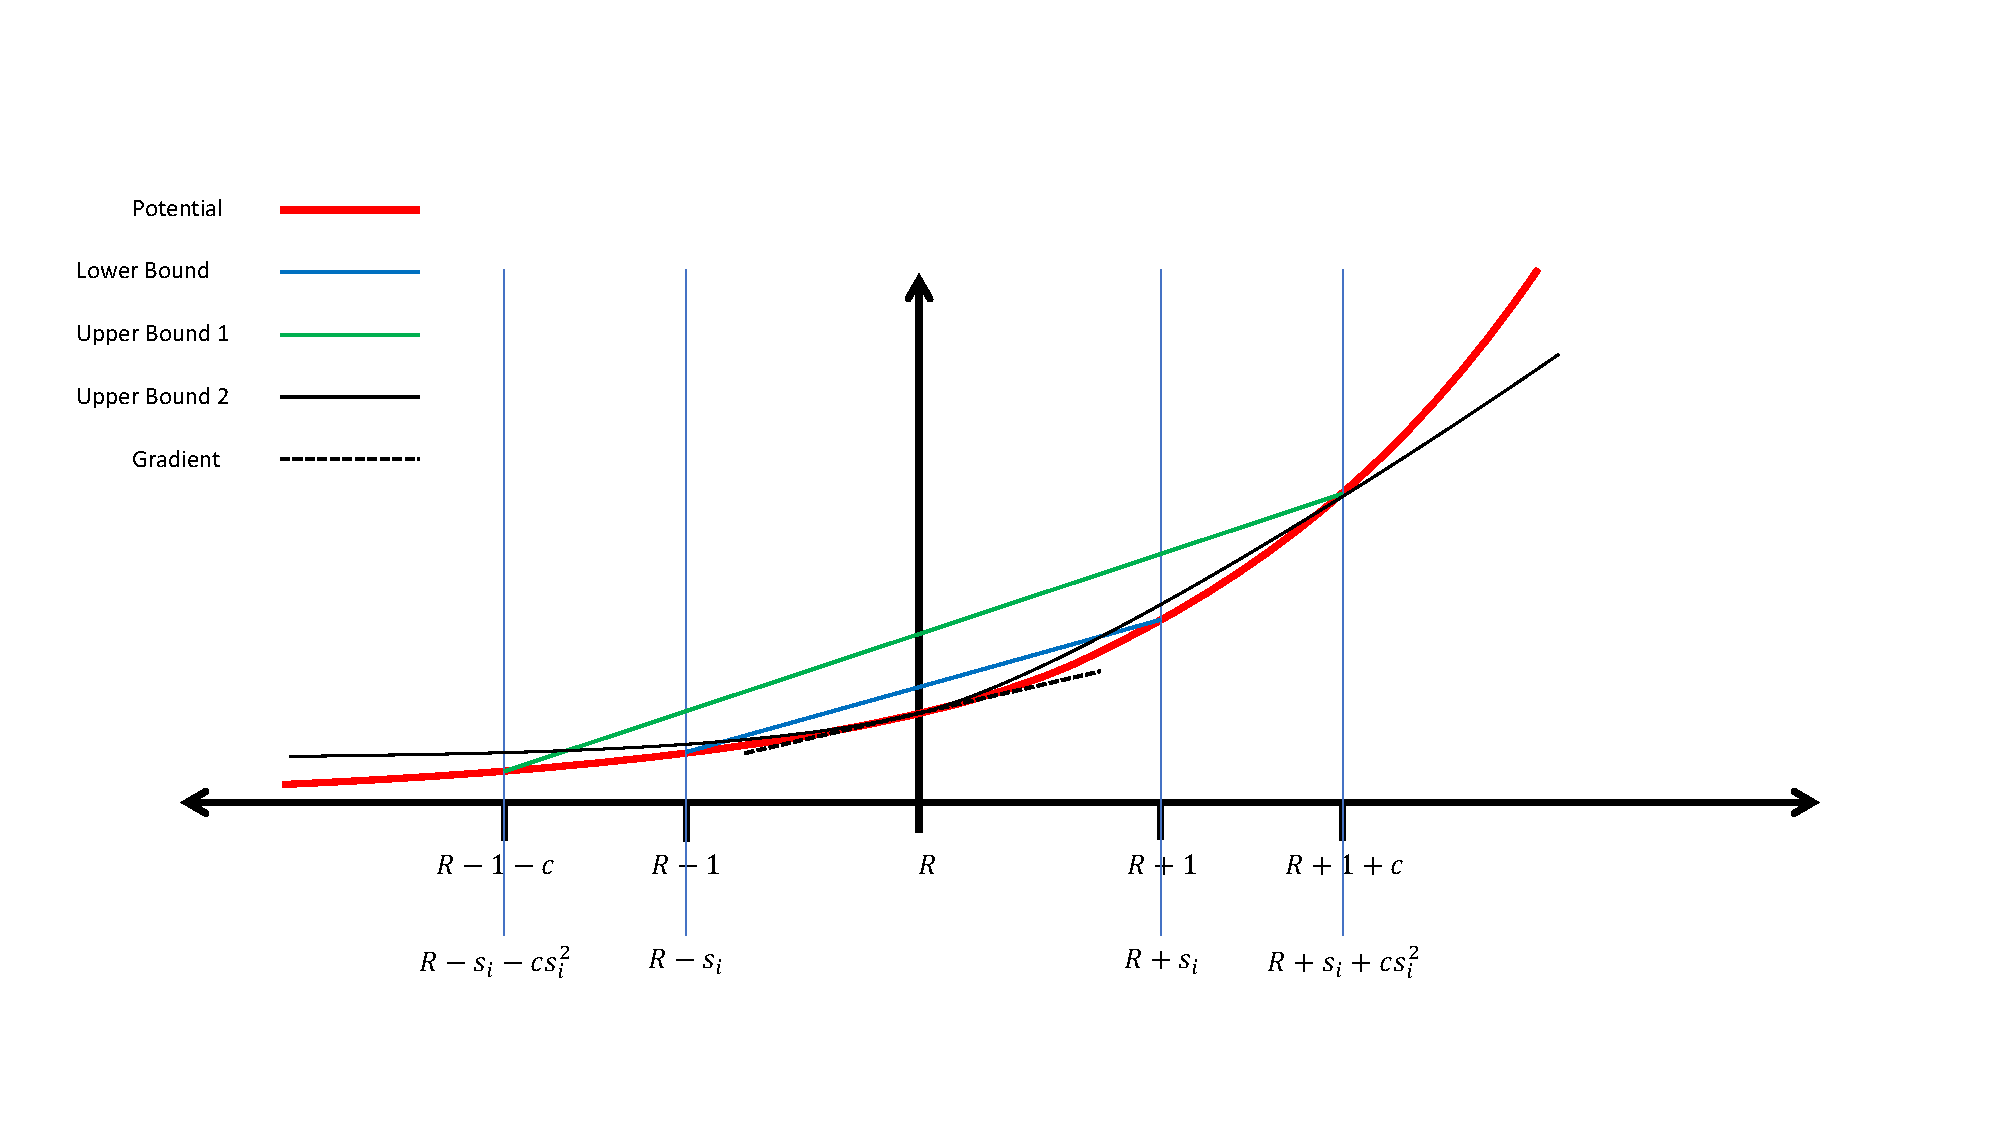
\includegraphics[width=\textwidth]{figures/convexPot.pdf}}
\caption{This figure depicts the relationship between the different
  upper and lower bounds used in the analysis. To aid understanding we
  describe the elements of the figure twice: once for the integer
  game, and once for the continuous time game. \newline
  {\bf Integer time game:} let
  the current iteration be $i$ and let the current regret be $\R$. Let
  $r$ be the regret at iteration $i+1$, we have that $\R-1-c \leq r
  \leq \R+1+c$. The
  potential at iteration $i+1$ is $\pot(i+1,r)$ (the red curve). The lower bound
  (blue line) corresponds to the adversarial strategy:
  $\adversM^{1/2}(i,\R)$. The first-order learner strategy:
  $\learnerM^1(i,\R)$ corresponds to the green line. The second-order
  learner strategy:  $\learnerM^2(i,\R)$ corresponds to the black
  curve.\newline
{\bf Continuous time game:} let
  the current iteration be $i$, the current time be $t_i$ and the
  current regret be $\R$. Let $0<s_i\leq 1$ be the step size chosen by the
  adversary, so that the next time is $t_{i+1} = t_i+s_i^2$. Let $r$
  be the regret at iteration
  $i+1$, we have that $\R-s_i-c s_i^2 \leq r \leq \R+s_i+c s_i^2$.
  The potential at iteration $i+1$ is $\pot(t_{i+1},r)$ (the red
  curve).  The lower bound (blue line) corresponds to the adversarial
  strategy: $\adversM^{1/2}_{\pm s_i}(t_i,\R)$. The first-order learner strategy:
  $\learnerM^{1c}(t_i,\R)$ corresponds to the green line. The second-order
  learner strategy: $\learnerM^{2c}(i,\R)$ corresponds to the black
  curve.   Observe that when $s_i \to 0$ the ratio $\frac{s_i}{s_i+c
    s_i^2}$ converges to 1, and the upper and gap between the green
  and blue lines converges to zero.\\
\rule[1ex]{6.5in}{0.5pt}}
\label{fig:ConvexPot}
\end{center}
\vskip -0.4in
\end{figure} 

  \subsection{A learner strategy with a variance-dependent bound}

  As shown in Lemma~\ref{lemma:adversary-prefers-extremes}, the
  adversary always prefers mixed strategies that assign zero
  probability for all steps other than $\pm 1$. Suppose, however, that
  the adversary is not worst-case optimal and chooses steps whose
  length is less than one. The following lemma gives a slightly
  different strategy for the learner, which guarantees a tighter bound
  for this case.

  \begin{lemma} \label{lemma:second-order-bound}
      The learner strategy:
      \begin{equation} \label{eqn:learner-strat-2}
      \learnerM^2(i-1,\R) =  \frac{1}{Z}
      \left. \frac{\partial}{\partial r} \right|_{r=\R} \pot(i,r)
      \end{equation}
      Where $Z$ is a normalization factor
      $$Z = \E{\R \sim \state(i)}{\left. \frac{\partial}{\partial r} \right|_{r=\R} \pot(i,r)}$$
      guarantees the following upper potential against any adversarial
      strategy $\adversM$
      \begin{equation} \label{eqn:value-iteration-upper}
        \upperpot(i-1, \R) = \pot(i,\R) + b(i,\R) \E{l \sim \adversM(i,\R)}{l^2}
      \end{equation}
      where $b(i,\R) = \pot(i,\R+1+c) -\pot(i,\R) - (1+c) \left. \frac{\partial}{\partial r} \right|_{r=\R} \pot(i,r)$
   \end{lemma}

We compare the bound for $\learnerM^2$ to the bound for $\learnerM^1$
given in Lemma~\ref{lemma:first-order-bound}. We find that when the 
adversary is optimal: $\E{l \sim \adversM(t,\R)}{l^2}=1$ then the
bound for $\learnerM^1$ is better than the bound for $\learnerM^2$, on the
other hand, when $\E{l \sim \adversM(t,\R)}{l^2}$ is close to zero,
$\learnerM^2$ is better than $\learnerM^1$.  

\section{Discrete time game}
\label{sec:discrete}

We start with motivation for using time that is indexed by real
values rather than the natural numbers. We distinguish between two
notions of time. The first notion of time is a counter that
counts the iterations of the game, we will call this counter the {\em
  iteration counter } and denote it by $i=0,1,\ldots$. The second,
more interesting notion of time is the time that appears in the regret
bounds, we denote this time by $t_i$ where $i$ is the iteration
number. We restrict the time increments $\Delta t_i =t_i-t_{i-1}$ to
the range $0\leq \Delta t_i \leq 1$.  The magnitude of $\deltat_i$
corresponds to the {\em hardness} of iteration $i$. $\deltat_i=0$
corresponds to the case where the losses of all of the strategies are
equal to a common value $-1 \leq a \leq 1$. In this case the aggregate
loss $\ell=a$, the state does not change:
$\state(i-1)=\state(i)$, $\Delta t_i=0$ and the instantanous regret is zero. On the
other hand $\Delta t_i=1$ corresponds to the adversarial strategy
$\adversM^{1/2}(t-1,R)$ (Eqn.~\ref{eqn:adv-strat}) which maximizes the
instantanous regret.

We introduce an additional step to the integer game. Before the
learner makes it's choice, the 
adversary chooses a real number $0 \leq s_i \leq 1$, by doing so, the
adversary commits that all of the instantanous expert lossesat that
step be in the range $[-s_i,s_i]$. The time step is defined to be $\deltat_i =
s_i^2$.

First, note that the adversary in this game is at least as powerful as
the adversary in the integer game. This is because the adversary can
always choose $s_i=1$, effectively reducing the game to the integer
game.

Next, we justify the choice $\deltat_i = s_i^2$. Our argument is that
any significantly different choice would give the game to one side or
the other.  Suppose that $s_i = 1/k$ on all $m_k$ iterations of the game. In
other words, this is a rescaling of the integer game. Consider the
adversarial strategy. The distribution (state) after $m_k$ iterations is the
binomial distribution. with mean zero and variance $m_k \frac{1}{k^2}$
if $m_k \gg \frac{1}{k^2}$ then the variance at the end of the game
goes to infinity.

\iffalse
The state after $m_k$ iterations is the
binomial dist
\begin{equation}
  \score^{m(k)} = \frac{1}{2^m} \sum_{i=-m}^m {2m+1 \choose i+m} \pot(m,i/k)
\end{equation}
if $m/\deltat_i $
\fi

By allowing $\Delta t_i$ to vary from iteration to iteration
we get a more refined quantification of the regret and, as we show
below, min/max optimality.

To find the relationship between loss magnitude and time increments 
we compare two adversarial strategies.  The first strategy, discussed above,
generates losses $\pm 1$ with equal probability, we deonte this
strategy by $\adversM^{1/2}_{\pm 1}$. The other strategy, denoted
$\adversM^{1/2}_{\pm 1/k}$, generates losses of $\pm 1/k$ with equal
probabilities.

From the adversarial point of view $\adversM^{1/2}_{\pm 1/k}$ is worse
than $\adversM^{1/2}_{\pm 1}$. So it should correspond to a smaller
time increment. But how much smaller? Suppose we start with the
initial state $\state(0)$ which is a delta functions at $\R=0$.  One
iteration of $\adversM^{1/2}_{\pm 1}$ results in a distribution
$\pm 1$ w.p, $(1/2,1/2)$, which has mean $0$ and variance $1$.
Suppose we associate $\Delta t =1/j$ with a single step of
$\adversM^{1/2}_{\pm 1/k}$.  Equivalently, we associate $j$ iterations
of $\adversM^{1/2}_{\pm 1/k}$ with $t=1$.  How should we set $j$? the
distribution generated by $j$ steps is a binomial distribution
supported on $j+1$ points, so there is no hope of making the two
distributions identical. However, as it turns out, it is enough to
equalize the mean and the variance of the two distributions. The mean
of $\adversM^{1/2}_{\pm 1/k}$ is zero for any $k$. As for the
variances, a single iteration of $\adversM^{1/2}_{\pm 1}$ is 1 and a
single iteration of $\adversM^{1/2}_{\pm 1/k}$ is $1/k^2$. It follows
that the variance after $j$ iterations of $\adversM^{1/2}_{\pm 1/k}$
$j/k^2$. Equating this variance with that of a single step of
$\adversM^{1/2}_{\pm 1}$ we get $j=k^2$ and $\Delta t= 1/k^2$.

Note a curious behaviour of the {\em range} of $\R$ as $k \to \infty$
the number of steps increases like $k^2$ while the size of each step
is $1/k$. This means that the range of $\R$ is $[-k,k]$, which becomes
converges to $(-\infty, + \infty)$ when $k \to \infty$. On the other
hand, the variance increases like $t$.

Next lets consider effect of reducing the step size on a {\em biased}
strategy $\adversM^{1/2+\gamma}_{\pm 1}$ as defined in
Eqn~(\ref{eqn:adv-strat-p}) for some
$0\leq \gamma \leq 1/2$.  We now figure out what  $\gamma'$ should be
so that the distribution generated by $k^2$ iterations of $\adversM^{1/2+\gamma'}_{\pm 1/k}$ has the
same mean as a single iteration of $\adversM^{1/2+\gamma}_{\pm
  1}$. The mean of a single iteration of
$\adversM^{1/2+\gamma}_{\pm 1}$ is $2\gamma$ while the mean of a
single iteration of $\adversM^{1/2+\gamma'}_{\pm 1/k}$ is
$2\gamma'/k$. Therefor to keep the means equal we need to set
$2\gamma'/k = 2\gamma$ or $\gamma' = \gamma/k$.


Note that as $k \to \infty$, $\gamma' \to 0$. This observation
motivates scaling the bound on $\ell(t)$ like $c s_i^2$ (see the
description of the game below.)



This leads to the following formulation of a continuous time game.
The game is a generalization of the integer time game in that it
reduces to the integer time game if the adversary always chooses $s_i=1$. 

In this game we use $i=1,2,3,\ldots$ as the iteration index. We use
$t_i$ to indicate a sequence of real-valued time points. $t_0=0$ and
we assume there exists a finite $n$ such that $t_n = T$.

We will later give some particular potential functions for which no
a-priori knowledge of the termination condition is needed. The
associated bounds will hold for any iteration of the game.
\vspace{1cm}

On iteration $i=1,2,\ldots$
\begin{enumerate}
\item  If $t_{i-1}=T$ the game terminates.
\item The adversay chooses a {\em step size} $0<s_i\leq 1$, which advances
  time by $t_i = t_{i-1}+s_i^2$.
\item Given $s_i$, the learner chooses a distribution $\learnerM(i)$ over $\reals$.
\item The adversary chooses a mapping from $\reals$ to distributions
  over $[-s_i,+s_i]$: $\adversM(t): \reals \to \Delta^{[-s_i,+s_i]}$
\item The aggregate loss is calculated:
  \begin{equation} \label{eqn:ell-discrete}
    \ell(t_i)=\E{\R \sim \state(t_i)}{\learnerM(t_i,\R)
      \Bias(t_i,\R)},\;\mbox{ where } \Bias(t_i,\R) \doteq \E{y \sim \adversM(t_i,\R)}{y}
  \end{equation}
\item the aggregate loss is restricted $|\ell(t_i)| \leq c s_i^2$.
\item The state is updated. The expectation below is over
  distributions. and the notation $G \oplus \R$ means
  that distribution $G$ over the reals is shifted by the amount
  defined by the scalar $\R$:
  $$\state(t_i) = \E{\R \sim \state(t_{i-1})}{\adversM(t_i)(\R)\oplus (\R-\ell(t_i))}
  $$
\end{enumerate}

When $t_i=T$ the game is terminated, and the final value is calculated:
$$\score(T) =\E{\R \sim \state(T)}{\finalPot(\R)}$$

\subsection{Results for the discrete time game}

In the discrete time game the adversary has an additional choice, the
choice of $s_i$. Thus the adversary's strategy includes that choice.
There are two constraints on this choice: $s_i \geq 0$ and
$\sum_{i=1}^n s_i^2 = T$. Note that even that by setting $s_i$
arbitrarily small, the adversary can make the number of steps - $n$ -
arbitrarily large. We will therefor not identify a single adversarial
strategy but instead consider the supremum over an infinite sequence
of strategies.

We use $N(0,\sigma)$ to denote the normal distribution with mean 0 and
std $\sigma$.

\begin{theorem}
  ~\\

   let $A = \E{\R \sim N(0,\sqrt{T})}{\pot(T,\R)}$
   \begin{itemize}
     \item
    For any $\epsilon>0$ there exists a strategy for the adversary
    such that for any strategy of the learner $\score(T) \geq A-\epsilon$
  \item
    There exists a strategy for the learner that guarantees, against
    any adversary $\score(T) \leq A$.
  \end{itemize}
\end{theorem}


\subsection{The adversary prefers smaller steps} \label{sec:smallsteps}
As noted before, if the adversary chooses $s_i=1$ for all $i$ the game
reduces the the integer time game. The question is whether the
adversary would prefer to stick with $s_i=1$ or instead prefer to use
$s_i<1$. In this section we give a surprising answer to this question
-- the adversary always prefers a smaller value of $s_i$ to a larger
one. This leads to a preference for $s_i \to 0$, as it turns out, this
limit is well defined and corrsponds to Brownian motion, also known as
Wiener process.

Consider a sequence of adversarial strategies $S_k$ indexed by
$k=0,1,2,$. The adversarial strategy $S_k$ is corresponds to always
choosing $s_i = 2^{-k}$, and repeating  $\adversM^{1/2}_{\pm 2^{-k}}$ 
for $T 2^{2k}$ iterations.
This corresponds to the distribution created by a random walk with
$T 2^{2k}$ time steps, each step equal to $+2^{-k}$ or  $-2^{-k}$ with probabilities $1/2,1/2$.
Note that in order to preserve the variance, halving the step size
requires incresing the number of iterations by a factor of four.

Let $\pot(S_k,t,\R)$ be the value associated with adversarial
strategy $S_k$, time $t$ (divisible by $2^{-2k}$) and
location $\R$. We are ready to state our main theorem.

\begin{theorem}\label{thm:smallerSteps}
  If the final value function has a strictly positive fourth
  derivative:
  $$ \frac{d^4}{d \R^4} \finalPot(\R) >0, \forall \R$$
  then for any integer $k>0$ and any $0 \leq  t \leq T$, such that $t$
  is divisible by
  $2^{-2k}$ and any $\R$,
  $$\pot(S_{k+1},t,\R)) >  \pot(S_{k},t,\R)$$
\end{theorem}

Before proving the theorem, we describe it's
consequence for the online learning problem.
We can restrict Theorem~\ref{thm:smallerSteps} for the
case $t=0$,$\R=0$ in which case we get an increasing sequence:
\[
\pot(S_1,0,0) < \pot(S_2,0,0) <\cdots <\pot(S_k,0,0) <
\]
The limit of the strategies $S_k$ as $k \to \infty$ is the well
studied Brownian or Wiener process. The backwards recursion that
defines the value function is the celebrated Backwrds Kolmogorov
Equation with zero dift and unit variance
\begin{equation} \label{eqn:Kolmogorov}
  \frac{\partial}{\partial t} \pot(t,\R)
  + \frac{1}{2} \frac{\partial^2}{\partial \R^2} \pot(t,\R)=0
\end{equation}
Given a final value function with a strictly positive fourth
derivative we can use Equation~(\ref{eqn:Kolmogorov}) to compute the
value function for all $0 \leq t \leq T$. We will do so in he next section.

We now go back to proving Theorem~\ref{thm:smallerSteps}. The core of
the proof is a lemma which compares, essentially, the value recursion
when taking one step of size 1 to four steps of size 1/2.


Consider the advesarial strategies $S_k$ and $S_{k+1}$ at a particular
time point $0 \leq t \leq T$ such that $t$ is divisible by
$\deltat=2^{-2k}$ and at a particular location $\R$. Let
$t'=t+\deltat$, and fix a value
function for time , $\pot(t',\R)$ and compare between
two values at $\R,t$. The first value denoted
$\pot_k(t,\R)$ corresponds to $S_k$, and consists of a single random step of $\pm 2^{-k}$. 
The other value $\pot_{k+1}(t,\R)$ corresponds to $S_{k+1}$ and consists of
four random steps of size $\pm 1/2$.

\begin{lemma} \label{lemma:n-strictly-convex}
If $\pot(t',\R)$ is, as a function of $\R$ continuous, strictly
convex and with a strictly positive fourth derivative. Then
\begin{itemize}
\item $\pot_k(t,\R) < \pot_{k+1}(t,\R)$
  \item Both $\pot_k(t,\R)$ and $\pot_{k+1}(t,\R)$ are continuous, strictly
convex and with a strictly positive fourth derivative.
\end{itemize}
\end{lemma}

\proof
Recall the notations $\deltat = 2^{-2k}$ $t' = t+\deltat$ and $s=2^{-k}$.
We can write out explicit expressions for the two values:
\begin{itemize}
\item For strategy $S_0$ the value is
  $$\pot_k(t, \R) = \frac{\pot(t',\R+s)+ \pot(t',\R-s)}{2} $$.
\item For strategy $S_1$ the value is
  $$\pot_{k+1}(t, \R) = \frac{1}{16}
  \paren{\pot(t',\R+2s)+ 4\pot(t',\R+s)+ 6\pot(t',\R)+  4\pot(t',\R-s)+ \pot(t',\R-2s)}
  $$.
\end{itemize}

We want to show that $\pot_1(T-1,\R) > \pot_0(T-1,\R)$ for all $\R$, in
other words we want to characterize the properties of $\finalPot$ the
would garantee that
\begin{equation}\label{eqn:4thOrderConvex}
\pot_1(t,\R) - \pot_0(t,\R) =
\frac{1}{16}
\paren{ \pot(t',\R+2) - 4\pot(t',\R+1) +6\pot(t',\R) - 4\pot(t',\R-1) +\pot(t',\R-2)} > 0
\end{equation}

Inequalities of this form have been studied extensively under the name
``divided differences''~\cite{popoviciu1965certaines,butt2016generalization, de2005divided}.
A function $\finalPot$ that satisfies
inequality~\ref{eqn:4thOrderConvex} is said to be {\em 4'th order convex}
(see details in in~\cite{butt2016generalization}).

$n$-convex functions have a very simple characterization:
\begin{theorem}
  Let $f$ be a  function with is differentiable up to order $n$, and
  let $f^{(n)}$ denote the $n$'th derivative, then $f$ is $n$-convex
  ($n$-strictly convex) if and only if $f^{(n)} \geq 0$ ($f^{(n)} > 0$).
\end{theorem}

We conclude that if $\pot(t',\R)$ has a strictly positive fourth
derivative then $\pot_{k+1}(t,\R) > \pot_{k}(t,\R)$ for all $\R$, proving
the first part of the lemma.

The second part of the lemma follows from the fact that
both $\pot_{k+1}(t,\R)$ and $\pot_{k}(t,\R)$ are convex combinations of
$\pot(t,\R)$ and therefor retain their continuity and convexity properties.

\qed

\proof  of Theorem~\ref{thm:smallerSteps} \\
The proof is by double induction over $k$ and over $t$.
For a fixed $k$ we take a finite backward induction over
$t=T-2^{-2k},T-2 \times 2^{-2k},T-3 \times 2^{-2k},\cdots,0$.
Our inductive claims are that $\pot_{k+1}(t,\R) > \pot_{k}(t,\R)$ and
$\pot_{k+1}(t,\R)$,$\pot_{k}(t,\R)$ are continuous, strongly convex and
have a strongly positive fourth derivative. That these claims carry over
from $t=T-i \times 2^{-2k}$ to  $t=T-(i+1) \times 2^{-2k}$ follows
directly from Lemma~\ref{lemma:n-strictly-convex}.

The theorem follows by forward induction on $k$.

\qed

\subsection{Strategies for the Learner in the discrete time game}
The strategies we propose for the learner in the continuous time game
are an adaptation of the strategies $\learnerM^1,\learnerM^2$ to the
case where $s_i<1$.

We start with the high-level idea. Consider iteration $i$ of the
continuous time game. We know that the adversary prefers $s_i$ to be
as small as possible. On the other hand, the adversary has to choose
some $s_i>0$. This means that the adversary always plays
sub-optimally. Based on $s_i$ the learner makes a choice and the
adversary makes a choice. As a result the current state $\state(t_{i-1})$
is transformed to $\state(t_i)$. To choose it's strategy, the learner
needs to assign value possible states $\state(t_i)$. How can she do
that? By assuming that in the future the adversary will play
optimally, i.e. setting $s_i$ arbitrarily small. While the adversary
cannot be optimal, it can get arbitrarily close to optimal, which is
brownian motion.

Solving the backwards Kolmogorov equation with the boundary condition
$\pot(T,\R)$ yields $\pot(t,\R)$ for any
$\R \in \reals$ and $t \in [0,T]$. We now explain how using this
potential function we derive strategies for the the learner. 

Note that the learner chooses a distribution {\em after} the adversary
set the value of $s_i$. The discrete time version of $\learnerM^1$
(Eqn~\ref{eqn:learner-strat-1}) is 
\begin{eqnarray} \label{eqn:learner-strat-1c}
  \learnerM^{1d}(t_{i-1},\R) = \frac{1}{Z^{1d}}
  \frac{\pot(t_i,\R+s_{i-1}+cs_{i-1}^2) -
  \pot(t_i,\R-s_{i-1}-cs_{i-1}^2)}{2} \\
  \mbox{ where } Z^{1d} = \E{\R \sim \state(t_i)}{\frac{\pot(t_i,\R+s_{i-1}+cs_{i-1}^2) -
  \pot(t_i,\R-s_{i-1}-cs_{i-1}^2)}{2}} \nonumber
\end{eqnarray}

Next, we consider the discrete time version of $\learnerM^2$:
(Eqn~\ref{eqn:learner-strat-2})
\begin{eqnarray} \label{eqn:learner-strat-2c}
  \learnerM^{2d}(t_{i-1},\R) =  \frac{1}{Z^{2d}}
  \left. \frac{\partial}{\partial r} \right|_{r=\R}
  \pot(t_{i-1}+s_{i-1}^2,r)
  \\
  \mbox{ where } Z^{2d} = \E{\R \sim
  \state(t_i)}{\left. \frac{\partial}{\partial r} \right|_{r=\R} \pot(t_{i-1}+s_{i-1}^2,r)} \nonumber
\end{eqnarray}

\section{Continuous time game} \label{sec:continuous}
In Section~\ref{sec:discrete} we have shown that the integer time game
has a natural extension to a setting where $\deltat_i = s_i^2$. We
also showed that the adversary gains from setting $s_i$ as small as
possible.
\iffalse
\begin{definition}[Continuous Time]
The continuous time limit is a sequence of games indexed by
$j=0,1,\ldots$. Suppose the stopping time for all games is equal to
$T$.
Let $s_i^j$ be the step size associated with the
$i'th$ iteration of game $j$. Then $s_i^j$ are supposed to have the
following properties:
\begin{itemize}
\item Let $s^j = \max_i s_i^j$, then $\lim_{j \to \infty} s^j = 0$
  \item for any $j$, $\sum_i (s_i^j)^2 = T$
\end{itemize}
  \end{definition}
\fi

We already have a worst case bound on this problem, which corresponds
to the adversary performing Brownian motion. Our goal here is to
refine this bound for the case where the adversary's strategies are not worst case.

To see that such an improvement is possible, consider the following
{\em constant} adversary. This adversary associates the same loss to
all experts on iteration $i$, formally, $\adversM(i,\R) = l$. In this
case the average loss is also equal to $l$, $\ell(i)=l$ which means
that all of the instantaneous regrets are $r=l-\ell(t_i) = 0$, which,
in turn, implies that $\state(i) = \state(i+1)$. As the state did not
change, it makes sense to set $t_{i+1}=t_i$, rather than
$t_{i+1}=t_i+s_i^2$.

We observe two extremes for the adversarial behaviour. The constant adversary for
which $t_{i+1} = t_i$, and the random walk adversary described
earlier, in which each expert is split into two, one half with loss
$-s_i$ and the other with loss $+s_i$. In which case $t_{i+1} =
t_i+s_i^2$. The analysis below shows that these are two extremes on a
spectrum and that intermediate cases can be characterized using a
variance-like quantity.

Our characterization applies to the limit where $s_i$ are small. Formally, we define
\begin{definition}
We say that an instance of the discrete time game is $(n,s,T)$-bounded if $\forall\;\; 0<i\leq n,\;\; s_i < s$ and $\sum_{i=1}^n s_i^2=T$
\end{definition}

We let $s \to 0$ keeping $\sum_i s_i^2 = T$. In this limit the strategy $\learnerM^{2c}$ (Equation~(\ref{eqn:learner-strat-2c}) simplifies to 
\begin{equation} \label{eqn:learner-strat-cc}
  \learnerM^{cc}(t,\R) =  \frac{1}{Z^{cc}}
  \left. \frac{\partial}{\partial r} \right|_{r=\R} \pot(t,r)
  \mbox{ where } Z^{cc} = \E{\R \sim \state(t_i)}{\left. \frac{\partial}{\partial r} \right|_{r=\R} \pot(t,r)}
\end{equation}


\begin{theorem} \label{thm:variancebound} Let $\pot \in \SP{\infty}$
  be a potential function that satisfies the Kolmogorov backward
  equation~(\ref{eqn:Kolmogorov}).  Let $T$ be fixed and let $G$ be an
  $(n,s,T)$-bounded instance of the discrete time game using $\pot$.
  Let the time increment associated with iteration $i$:
  $\deltat_i = t_{i+1} - t_i$ be set so that
\begin{equation} \label{eqn:deltat}
  \deltat_i= 
  \E{\R \sim \state(t_i)}{\E{y \sim \adversM(t_i,R)}{G(t_i,\R)
      (y-\ell(t_i))^2}} 
\end{equation}
Where
\[
  G(t,\R) = \frac{1}{Z^G}
      \left. \frac{\partial^2}{\partial \rho^2} \right|_{\rho=\R} \pot(t,\rho)
,\;\; Z^G=\E{\R \sim \state(t_i)}{\left. \frac{\partial^2}{\partial \rho^2} \right|_{\rho=\R} \pot(t,\rho)}
    \]
then 
$$\score(\state(0)) \leq \score(\state(T))+O(sT)$$
\end{theorem}

The proof of the theorem is given in appendix~\ref{appendix:ProofOfVarianceBound}

Theorem~\ref{thm:variancebound} shows that the average potential does
not stay constant, instead, it increases by at most $O(s^3)$ at each
iteration. As $T$ increases by at most $s^2$ at each iteration we find
that the total increasein the potential is at most $Ts$. 

  
%    \E{\R \sim \state(i-1)}{ \E{y \sim
%      \adversM(i-1)(\R)}{\pot(i,\R+y-\ell(i-1))}}

\section{Two self-consistent potential functions} \label{sec:self-consistent}

The potential functions, $\pot(t,\R)$ is a solution of PDE~(\ref
{eqn:Kolmogorov}):
\begin{equation} 
  \frac{\partial}{\partial t} \pot(t,\R)
  + \frac{1}{2} \frac{\partial^2}{\partial r^2} \pot(t,\R)=0
\end{equation}
under a boundary condition $\pot(T,\R)=\finalPot(\R)$, which we assume
is in $\SP{4}$

So far, we assumed that the game horizon $T$ is known in advance. We
now show two value functions where knowledge of the horizon is not
required. Specifically, we call a value function $\pot(t,\R)$
{\em self consistent} if it is defined for all $t>0$ and if for any
$0<t<T$, setting $\phi(T,\R)$ as the final potential and solving for
the Kolmogorov Backward Equation yields $\phi(t,\R)$ regarless of the
time horizon $T$. 

We consider two solutions to the PDE, the exponential potential and
the NormalHedge potential. We give the form of the potential function
that satisfies Kolmogorov Equation~\ref{eqn:Kolmogorov}, and derive
the regret bound corresponding to it.

{\bf The exponential potential function} which corresponds to exponential
  weights algorithm corresponds to the following equation
\[
    \pot_{\mbox{exp}}(\R,t) = e^{\sqrt{2} \eta \R - \eta^2 t}
  \]
  Where $\eta>0$ is the learning rate parameter.
  
Given $\epsilon$ we choose $\eta = \sqrt{\frac{\ln (1/\epsilon)}{t}}$
we get the regret bound that holds for any $t>0$
  \begin{equation}
    \R_\epsilon \leq \sqrt{2 t \ln \frac{1}{\epsilon}}
  \end{equation}
Note that the algorithm depends on the choice of $\epsilon$, in other
words, the bound does {\em not} hold for all values of $\epsilon$ at
the same time.

{\bf The NormalHedge value} is
\begin{equation} \label{eqn:NormalHedge}
  \pot_{\mbox{NH}}(\R,t) = \begin{cases}
    \frac{1}{\sqrt{t+\nu}}\exp\left(\frac{\R^2}{2(t+\nu)}\right)
    & \mbox{if } \R \geq 0  \\
  \frac{1}{\sqrt{t+\nu}} & \mbox{if } \R <0
  \end{cases}
\end{equation}
Where $\nu>0$ is a small constant. The function $\pot_{\mbox{NH}}(\R,t)$,
restricted to $\R\geq 0$ is in $\SP{4}$ and is a constant for $\R \leq 0$.

The regret bound we get is:
\begin{equation}
\R_\epsilon \leq \sqrt{(t+\nu) \left( \ln (t+\nu) + 2 \ln \frac{1}{\epsilon}\right)}
\end{equation}
This bound is slightly larger than the bound for exponential weights,
however, the NormalHedge bound holds simultanuously for all
$\epsilon>0$ and the algorithm requires no tuning.


\section{NormalHedge yields the fastest increasing potential} \label{sec:NormalHedge}

Up to this point, we considered any continuous value function with
strictly positive derivatives 1-4. We characterized the min-max
strategies for any such function. It is time to ask whether value
functions can be compared and whether there is a ``best'' value
function. In this section we give an informal argument that
NormalHedge is the best function. We hope this argument can be
formalized.

We make two observations. First, the min-max strategy for the
adversary does not depend on the potential function! (as long as it
has strictly positive derivatives). That strategy corresponds to the
brownian process.

Second, the argument used to show that the regret relative to
$\epsilon$-fraction of the expert is based on two arguments
\begin{itemize}
\item The average value function does not increase with time.
\item The (final) value function increases rapidly as a function of $\R$
\end{itemize}
The first item is true by construction. The second argument suggests
the following partial order on value functions. Let
$\pot_1(t,\R),\pot_2(t,\R)$ be two value functions such that
\[
\lim_{\R \to \infty} \frac{\pot_1(t,\R)}{\pot_2(t,\R)} = \infty  
\]
then $\pot_1$ {\em dominates} $\pot_2$, which we denote by, $\pot_1 > \pot_2$.

On the other hand, if the value function increases too quickly, then,
when playing against brownian motion, the average value will increase
without bound.  Recall that the distribution of the brownian process
at time $t$ is the standard normal with mean 0 and variance $t$.
The question becomes what is the fastest the value
function can grow, as a function of $\R$ and still have a finite
expected value with respect to the normal distribution.

The answer seems to be NormalHedge (Eqn.~\ref{eqn:NormalHedge}). More
precisely, if $\epsilon>0$, the mean value is finite, but if
$\epsilon=0$ the mean value becomes infinite.

\bibliographystyle{plain}
\bibliography{ref.bib}

\appendix
\section{Proof of Theorem~\ref{thm:variancebound}}
\label{appendix:ProofOfVarianceBound}
We start with two technical lemmas
\begin{lemma} \label{lemma:infiniteexpectations}
Let $f(x) \in \SP{2}$, i.e. $f(x), f'(x),f''(x) >0$ for all $x \in
\reals$, let $h(x)$ be a uniformly bounded function: $\forall x,\;\; |h(x)|<1$.
Let $\state$ be a distribution over $\reals$.
If $\E{x \sim \state}{f(x)}$ is well-defined (and finite) , then 
$\E{x \sim \state}{h(x) f'(x)}$ is well defined (and finite) as well.
\end{lemma}
\proof
Assume by contradiction that $\E{x \sim \state}{h(x) f'(x)}$ is
undefined. Define $h^+(x) = \max(0,h(x))$.
As $f'(x)>0$, this implies that either $\E{x \sim \state}{h^+(x)
  f'(x)}=\infty$ or $\E{x \sim \state}{(-h)^+(x) f'(x)}=\infty$ (or both). 

Assue wlog that $\E{x \sim \state}{h^+(x) f'(x)}=\infty$. As
$f'(x)>0$ and $0 \leq h^+(x) \leq 1$ we get that $\E{x \sim
  \state}{f'(x)}=\infty$.
As $f(x+1) \geq f'(x)$ we get that $\E{x \sim
  \state}{f(x)}=\infty$ which is a contradiction.
\qed

\iffalse
$\epsilon>0$ such that
for any $v>0$ there exists $|h_v(x)| < v$ such that 
$|\E{x \sim \state}{h_v(x) f'(x)}|>\epsilon$. Define $h'_v =
\frac{h_v}{v}$. Clearly $|h'_v(x)|<1$ and we have that
$$|\E{x \sim \state}{h'_v(x) f'(x)}|>\frac{\epsilon}{v}$$

Define the positive parts of $h_v$ to be $h_v^+(x) = \max(0,h'_v(x))$
and $h_v^-(x) = \max(0,-h'_v(x))$. As $f'(x)>0$ we that either
\[
  \E{x \sim \state}{h^+_v(x) f'(x)}>\frac{\epsilon}{v}
\]
or 
\[
  \E{x \sim \state}{h^-_v(x) f'(x)}>\frac{\epsilon}{v}
\]
Wlog assume the first. As $f \in \SP{2}$, we have that $f(x+1) \geq f'(x)$. Therefore
 $\E{x \sim \state}{f(x+1)|h_v^(x)>0)}=\infty$. As $f(x)>0$ for all $x$ we
 find that $\E{x \sim \state}{f(x)}=\infty$ which contradicts the
 Lemma's assumption.
\qed
\fi

\newcommand{\Dx}{\Delta x}
\newcommand{\Dy}{\Delta y}
\begin{lemma} \label{lemma:Taylor2D}
Let $f(x,y)$ be a differentiable function with continuous derivatives
up to degree three. Then
\begin{eqnarray}
  &&f(x_0+\Dx,y_0+\Dy) = f(x_0,y_0)
  + \atI{\frac{\partial}{\partial x}} \Dx 
  + \atI{\frac{\partial}{\partial y}} \Dy \\
  &+&\frac{1}{2} \atI{\frac{\partial^2}{\partial x^2}} \Dx^2
      +\atI{\frac{\partial^2}{\partial x\partial y}} \Dx\Dy
      +\frac{1}{2} \atI{\frac{\partial^2}{\partial y^2}} \Dy^2\\
  &+&\frac{1}{6} \atII{\frac{\partial^3}{\partial x^3}} \Dx^3
      +\frac{1}{2} \atII{\frac{\partial^3}{\partial x^2 \partial y}} \Dx^2\Dy\\
  &&+ \frac{1}{2} \atII{\frac{\partial^3}{\partial x \partial y^2}} \Dx\Dy^2
    + \frac{1}{6} \atII{\frac{\partial^3}{\partial y^3}} \Dy^3
\end{eqnarray}
for some $0\leq t \leq 1$.
\end{lemma}
\proof {\em of Lemma~\ref{lemma:Taylor2D}} 
Let $F:[0,1] \to \reals$ be defined as  $F(t)=f(x(t),y(t))$ where
$x(t) = x_0+t\Dx$ and $y(t)=y_0+t\Dy$. Then $F(0)=f(x_0,y_0)$ and
$F(1)=f(x_0+\Dx,y_0+\Dy)$. It is easy to verify that
$$ \frac{d}{dt}F(t)
=\frac{\partial}{\partial x} f(x(t),y(t))\Dx
+ \frac{\partial}{\partial y} f(x(t),y(t))\Dy
$$
and that in general:
\begin{equation} \label{eqn:d.dn.F}
\frac{d^n}{d t^n} F(t) = \sum_{m=1}^n {n \choose m}
\frac{\partial^n}{\partial x^m \partial y^{n-m}} f(x_0+t \Dx,y_0+t\Dy)
\Dx^m \Dy^{n-m}
\end{equation}
As $f$ has partial derivatives up to degree 3, so does $F$. Using the
Taylor expansion of $F$ and the intermediate point theorem we get that
\begin{equation} \label{eqn:Taylor.F}
  f(x_0+\Dx,y_0+\Dy) = F(1) = F(0)+\frac{d}{dt}F(0)
  +\frac{1}{2}\frac{d^2}{dt^2}F(0)
  +\frac{1}{6}\frac{d^3}{dt^3}F(t')
\end{equation}
Where $0 \leq t' \leq 1$. Using Eqn~(\ref{eqn:d.dn.F}) to expand each
term in Eqn.~(\ref{eqn:Taylor.F}) completes the proof.
\qed


\proof {\em of Theorem~\ref{thm:variancebound}}\\
We prove the claim by an upper bound on the increase of potential that holds for any iteration $1 \leq i \leq n$:
\begin{equation} \label{proof:onestep}
\score(\state(t_{i+1})) \leq \score(\state(t_i)) + a s_i^3 \mbox{ for some constant } a>0
\end{equation}
Summing inequality~(\ref{proof:onestep}) over all iterations we get that 
\begin{equation} \label{proof:allsteps}
\score(\state(T)) \leq \score(\state(0)) + c \sum_{i=1}^n s_i^3 \leq 
\score(\state(0)) + a s \sum_{i=1}^n s_i^2 = 
\score(\state(0)) + a s T
\end{equation}
From which the statement of the theorem follows.

We now prove inequality~(\ref{proof:onestep}). 
We use the notation $r=y -\ell(i)$ to denote the instantaneous regret at iteration $i$. 


Applying Lemma~\ref{lemma:Taylor2D} to
$\pot(t_{i+1},\R_{i+1})=\pot(t_i+\deltat_i,\R_i+r_i)$  we get
\begin{eqnarray} 
    \pot(t_i+\deltat_i,\R_i+r_i) & =&  
    \pot(t_i,\R_i)\\
    &+&\at{\frac{\partial}{\partial \rho}} r_i \\
    &+&\at{\frac{\partial}{\partial \tau}}  \deltat_i \\
    &+& \frac{1}{2} \at{\frac{\partial^2}{\partial \rho^2}} r_i^2 \\
    &+& \at{\frac{\partial^2}{\partial r \partial \tau}} r_i \deltat_i \label{term:Taylor_rdt}\\
    &+& \frac{1}{2} \at{\frac{\partial^2}{\partial \tau^2}} \deltat_i^2 \label{term:Taylor_dtsquare}\\
    &+& \frac{1}{6} \att{\frac{\partial^3}{\partial \rho^3}} r_i^3 \label{term:Taylor_r3}\\
    &+& \frac{1}{2} \att{\frac{\partial^3}{\partial \rho^2 \partial \tau}} r_i^2\deltat_i \label{term:Taylor_r2t}\\
    &+& \frac{1}{2} \att{\frac{\partial^3}{\partial \rho \partial \tau^2}} r_i\deltat_i^2 \label{term:Taylor_rt2}\\
    &+& \frac{1}{6} \att{\frac{\partial^3}{\partial \tau^3}} \deltat_i^3 \label{term:Taylor_t3}
\end{eqnarray}
for some $0 \leq g \leq 1$.

By assumption $\pot$ satisfies the Kolmogorov backward equation:
\begin{equation*} 
  \frac{\partial}{\partial \tau} \pot(\tau,\rho)
  = -\frac{1}{2} \frac{\partial^2}{\partial r^2} \pot(\tau,\rho)
\end{equation*}
Combining this equation with the exchangability of the order of
partial derivative (Clairiaut's Theorem) we can substitute all
partial derivatives with respect to $\tau$ with partial derivatives
with respect to $\rho$ using the following equation.
\[
  \frac{\partial^{n+m}}{\partial \rho^n \partial \tau^m} \pot(\tau,\rho)=
  (-1)^m \frac{\partial^{n+2m}}{\partial \rho^{n+2m}} \pot(\tau,\rho)
\]
Which yields
\begin{eqnarray}
      \pot(t_i+\deltat_i,\R_i+r_i) & =&  
    \pot(t_i,\R_i)\\
    &+& \at{\frac{\partial}{\partial \rho}} r_i \label{term:coll1}\\
    &+& \at{\frac{\partial^2}{\partial \rho^2}} \paren{\frac{r_i^2}{2}-\deltat_i} \label{term:coll2}\\
    &-& \at{\frac{\partial^3}{\partial \rho^3}} r_i \deltat_i \label{term:coll3}\\
    &+& \frac{1}{2} \at{\frac{\partial^4}{\partial \rho^4}} \deltat_i^2 \label{term:coll4}\\
    &+& \frac{1}{6} \att{\frac{\partial^3}{\partial \rho^3}} r_i^3 \label{term:coll5}\\
    &-& \frac{1}{2} \att{\frac{\partial^4}{\partial \rho^4}} r_i^2\deltat_i \label{term:coll6}\\
    &+& \frac{1}{2} \att{\frac{\partial^5}{\partial \rho^5}} r_i\deltat_i^2 \label{term:coll7}\\
    &-& \frac{1}{6} \att{\frac{\partial^6}{\partial \rho^6}} \deltat_i^3 \label{term:coll8}
\end{eqnarray}

  From the assumption that the game is $(n,s,T)$-bounded we get that 
  \begin{enumerate}
  \item $|r_i| \leq s_i +c s_i^2 \leq 2 s_i$
  \item $\deltat_i \leq s_i^2 \leq s^2$
    % \item $\sum_i \deltat_i=T$
  \end{enumerate}

  given these inequalities we can rewrite the second factor in each
  term as follows, where $|h_i(\cdot)|\leq 1$
  \begin{itemize}
  \item {\bf For~(\ref{term:coll1}):}
    $r_i=2s_i\frac{r_i}{2s_i}=2s_ih_1(r_i)$.
  \item {\bf For~(\ref{term:coll2}):}
    $r_i^2 - \frac{1}{2}\deltat_i = 4s_i^2\frac{r_i^2 -
      \frac{1}{2}\deltat_i}{4s_i^2} = 4s_i^2 h_2(r_i,\deltat_i)$
  \item {\bf For~(\ref{term:coll3}):} $r_i \deltat_i = 2s_i^3
    \frac{r_i \deltat_i}{2s_i^3} = 2s_i^3 h_3(r_i,\deltat_i)$
  \item {\bf For~(\ref{term:coll4}):} $\deltat_i^2 =
    s_i^4\frac{\deltat_i^2}{s_i^4} = s_i^3 h_4(\deltat_i)$
  \item {\bf For~(\ref{term:coll5}):} $r_i^3 = 8s_i^3
    \frac{r_i^3}{8s_i^3} = 8s_i^3 h_5(r_i,\deltat_i)$
  \item {\bf For~(\ref{term:coll6}):} $r_i^2 \deltat_i = 4s_i^4
    \frac{r_i^2 \deltat_i}{4s_i^4} = 4s_i^3 h_6(r_i,\deltat_i)$
  \item {\bf For~(\ref{term:coll7}):} $r_i \deltat_i^2 = 2s_i^5
    \frac{r_i \deltat_i^2}{2s_i^5}$
  \item {\bf For~(\ref{term:coll8}):} $\deltat_i^3 = s_i^6 \frac{\deltat_i^3}{s_i^6}$
\end{itemize}
  We therefor get the simplified equation
  
  \begin{eqnarray*} 
     \pot(t_i+\deltat_i,\R_i+r_i) & =&  \pot(t,\R)+\at{\frac{\partial}{\partial r}} r
    + \at{\frac{\partial}{\partial t}} \deltat \\
                                  &+& 
                                      \frac{1}{2}  \at{\frac{\partial^2}{\partial r^2}} r^2\\
                                  &+& \at{\frac{\partial^2}{\partial r \partial t}} r_i \deltat_i \label{term:Taylor_collected_rdt}\\
                                  &+& \frac{1}{6} \at{\frac{\partial^3}{\partial r^3}} r_i^3 \label{term:Taylor_collected_r3}
                                      + O(s^4)
\end{eqnarray*}

and therefor
  \begin{eqnarray} 
     \pot(t_i+\deltat_i,\R+r) &=& \pot(t_i,\R) +
                                  \at{\frac{\partial}{\partial r}} r
                                  \nonumber \\
    &+& \at{\frac{\partial^2}{\partial r^2}} (r^2 - \deltat_i) +
        O(s^3) \label{eqn:Taylor}
\end{eqnarray}

Our next step is to consider the expected value of~(\ref{eqn:Taylor}) wrt $\R \sim \state(t_i)$,
$y \sim \adversM(t_i,\R)$ for an arbitrary adversarial strategy
$\adversM$.

We will show that the expected potential does not increase:
\begin{equation} \label{eqn:deltatislargeenough}
     \E{\R \sim \state(t_i)}{ \E{y \sim \adversM(t_i,\R)}{\pot(t_i+\deltat_i,\R+y-\ell(t_i))}} \leq \E{\R \sim \state(t_i)}{\pot(t_i,\R)}
\end{equation}

Plugging Eqn~(\ref{eqn:Taylor}) into the LHS of
Eqn~(\ref{eqn:deltatislargeenough}) we get
\begin{eqnarray}
  \lefteqn{\E{\R \sim \state(t_i)}{\E{y \sim \adversM(t_i,\R)}{\pot(t_i+\deltat_i,\R+y-\ell(t_i))}}} \\
  &=& \E{\R \sim \state(t_i)}{\pot(t_i,\R)} \label{eqn:contin0}\\
  &+& \E{\R \sim \state(t_i)}{\E{y \sim \adversM(t_i,\R)}{\at{\frac{\partial}{\partial r}} (y-\ell(t_i))}} \label{eqn:contin1}\\
  &+& \E{\R \sim \state(t_i)}{\E{y \sim
      \adversM(t_i,\R)}{\at{\frac{\partial^2}{\partial r^2}}
      ((y-\ell(t_i))^2 - \deltat_i)}}
  \label{eqn:contin2}\\
  &+& O(s^3) \label{eqn:contin3}
\end{eqnarray}
Some care is needed here. we need to show that the expected value
are all finite. We assume that the expected potential
(Eqn~({eqn:contin0}) is finite. Using
Lemma~\ref{lemma:infiniteexpectations} this implies that the expected
value of higher derivatives of $\frac{\partial}{\partial \R} \pot(\R)$
are also finite.\footnote{I need to clean this up and find an argument
  that the expected value for mixed derivatives is also finite.}


To prove inequality~(\ref{proof:onestep}), we need to show that the
terms~\ref{eqn:contin1} and \ref{eqn:contin2} are smaller or equal to
zero.
~\\~\\~\\
{\bf Term~(\ref{eqn:contin1}) is equal to zero:}\\
As $\ell(t_i)$ is a constant
relative to $\R$ and $y$, and $\at{\frac{\partial}{\partial r}}$ is a
constant with respect to $y$ we can rewrite~(\ref{eqn:contin1}) as
\begin{equation} \label{eqnterm1.1}
  \E{\R \sim \state(t_i)}{\at{\frac{\partial}{\partial r}}
    \E{y \sim \adversM(t_i,\R)}{y} }
- \ell(t_i) \E{\R \sim \state(t_i)}{\at{\frac{\partial}{\partial r}}}
\end{equation}

Combining the definitions of $\ell(t)$~(\ref{eqn:ell-discrete}) and~
and the learner's strategy
$\learnerM^{cc}$~(\ref{eqn:learner-strat-cc}) we get that
\begin{eqnarray}
\ell(t_i) &=& \E{\R \sim \state{t_i}}{\frac{1}{Z}
              \at{\frac{\partial}{\partial r}}
              \E{y \sim \adversM(i,\R)}{y}} \mbox{ where }
              Z=\E{\R \sim \state{t_i}}{\frac{1}{Z}
              \at{\frac{\partial}{\partial r}}}
              \label{eqnterm1.2}
\end{eqnarray}

Plugging~(\ref{eqnterm1.2}) into (\ref{eqnterm1.1}) and recalling the
requirement that $\ell(t_i)<\infty$ we find that
term~(\ref{eqn:contin1}) is equal to zero.


~\\~\\~\\
{\bf Term~(\ref{eqn:contin2}) is equal to zero:}\\
As $\deltat_i$ is a constant relative to $y$, we can take it
outside the expectaation to give 
\begin{equation} \label{eqn:term2.1}
  \E{\R \sim \state(t_i)}{\E{y \sim
      \adversM(t_i,\R)}{\at{\frac{\partial^2}{\partial r^2}}
      (y-\ell(t_i))^2}}
  - \deltat_i  \;  \E{\R \sim \state(t_i)}{\at{\frac{\partial^2}{\partial r^2}}}
\end{equation}
On the other hand, from the choice of $\deltat_i$ given in
Eqn~(\ref{eqn:deltat}) we get
\begin{equation} \label{eqn:term2.2}
  \deltat_i \; \E{\R \sim \state(t_i)}{\at{\frac{\partial^2}{\partial r^2}}} = 
  \E{\R \sim \state(t_i)}{\E{y \sim \adversM(t_i,R)}{
      \at{\frac{\partial^2}{\partial r^2}} (y-\ell(t_i))^2}}
\end{equation}
Combining~(\label{eqn:term2.1}) and~(\ref{eqn:term2.2}) we
find that (\ref{eqn:contin2}) is zero.

Finally (\ref{eqn:contin3}) is negligible relative to the other terms
as $s \to 0$.
\qed 

\end{document}


